%%%%%%%%%%%%%%%%%%%%%%%%%%% asme2ej.tex %%%%%%%%%%%%%%%%%%%%%%%%%%%%%%%

%%%%%%%%%%%%%%%%%%%%%%%%%%%%%%%%%%%%%%%%%%%%%%%%%%%%%%%%%%%%%%%%%%%%%%

%%% use twocolumn and 10pt options with the asme2ej format
\documentclass[twocolumn,10pt]{asme2ej}
%
\usepackage{epsfig} %% for loading postscript figures

%% The class has several options
%  onecolumn/twocolumn - format for one or two columns per page
%  10pt/11pt/12pt - use 10, 11, or 12 point font
%  oneside/twoside - format for oneside/twosided printing
%  final/draft - format for final/draft copy
%  cleanfoot - take out copyright info in footer leave page number
%  cleanhead - take out the conference banner on the title page
%  titlepage/notitlepage - put in titlepage or leave out titlepage
%
%% The default is oneside, onecolumn, 10pt, final


\title{MATH 371 Fall Quarter MCM 2019 Problem B}


\begin{document}

\maketitle


\begin{abstract}
{\it This is the abstract. This is the thing we're going to spend a LOT of time writing, it's very important. We still need to write the abstract and the introduction
}
\end{abstract}

%\begin{nomenclature}
%\entry{A}{You may include nomenclature here.}
%\entry{$\alpha$}{There are two arguments for each entry of the nomemclature environment, the symbol and the definition.}
%\end{nomenclature}

%The primary text heading is  boldface and flushed left with the left margin.  The spacing between the  text and the %heading is two line spaces.

\section{Introduction}

This is the introduction

\section{Ideation}
We identified two significant problems to focus on in our model: packaging the drones and medi-packs to be deployed in the disaster area, and routing the drones to deliver necessary supplies according to the requirements from the delivery locations in attachment 4. We generalized a solution early on that involved algorithmically optimizing the packing space in each cargo container and modeling many routes to choose an ideal route based on a cost function, thereby eliminating two degrees of freedom. The remaining freedom is in choosing which drone type to use, which we determined could be implemented in the flight-path algorithm.

In this problem, there is already a lot of information established: the dimensions of all interacting products are fully defined, the performance capabilities of the drones are known, and the exact locations of delivery locations in the form of latitude and longitude points are provided. We used all this information to our advantage to narrow the scope of the problem and allow us more time to model the specific operational flow of our disaster response system. Despite this, however, several assumptions and simplifications were made in our model to reduce complexity which are outlined below.

\section{Assumptions}

\begin{itemize}
	\item Scheduling
	\begin{itemize}
		\item[--] Only the minimum supplies required daily are delivered to delivery locations, i.e. no rotating schedules and stockpiling of supplies to avoid needing to deliver to each daily
		\item[--] Additional time for operations is not considered: no time is needed to be spent in between flights for loading supplies or recharging the drones, and no time is needed to land and deliver supplies at delivery locations
	\end{itemize}
    \item Packing
    \begin{itemize}
    	\item[--] Elements can be stacked in any configuration without structural limitations
    \end{itemize}
	\item Flight path routing
	\begin{itemize}
		\item[--] Paths are perfectly straight
		\item[--] Every path only has either the delivery location or storage container as origin and destination
		\item[--] Paths are modeled in two dimensions i.e. no altitude changes are considered
		\item[--] Not considering effects of having multiple drones flying at once
	\end{itemize}
	\item Environmental effects
	\begin{itemize}
		\item[--] Influences from wind are neglected
		\item[--] The drones are assumed to be unobstructed by terrain
		\item[--] The drones do not experience any malfunctions
		\item[--] The earth’s curve is neglected
	\end{itemize}
\end{itemize}


\section{Overview of Algorithms}
 
 
\subsection{Flight Path Algorithm}
The flight path algorithm inputs the coordinates of each delivery location and its required medi-packs, information about each drone type, and assumes the starting location to be (0,0). It generates a list of all possible configurations of flight paths, each one represented as a vector of 2D lines. Any configurations that do not visit required hospitals , otherwise fail to meet delivery requirements, or cannot be sufficiently packed into the storage container(s) are eliminated from the list. A cost function that divides the total number of packages delivered by total distance over maximum speed is applied to the remaining list of configurations to find the least expensive flight paths. The algorithm is written in MATLAB and outputs a graph which represents the flight paths as lines and delivery locations as points, and the program outputs the total number of optimized flight paths found in the console.

The algorithm does not apply any calculation to determine how many medi-packs can fit in each drone configuration: analysis was done by hand to evaluate this for each drone type, and the maximum number of medi-packs that each drone can carry is hardcoded into the algorithm. 

Many limitations from this algorithm become immediately apparent: the real-life terrain that would be faced by the drones is ignored in favor of an ultra-simple “by the crow flies” model of flight. By utilizing this approach, the model also invalidates any capability of maximizing surveillance of roadways on the island of Puerto Rico, which was identified as a major focus for the DroneGo disaster response system.

\subsection{Packing Algorithm}
A packing algorithm is used to determine whether the materials necessitated by each flight configuration can be spatially packed into the dimensions of a standard ISO dry cargo container. The algorithm inputs the dimensions of each drone type and each medipack, and outputs a simple boolean expressing whether the configuration will fit or not. The algorithm  inputs the items into the cargo area by creating columns with base dimensions defined by the packages, and checks whether each new package can be stacked in an existing column before resorting to making a new column. Each package is only considered for one optimal orientation which is hardcoded prior. If the algorithm still has packages left to pack, but cannot create any more columns, it will return a 0.

\subsection{Cost Function}
Our cost function is described by the following formula, evaluating for a via flight plan and drone configuration.
\[
C = \alpha \frac{P}{\sum{t}} - \beta \frac{S}{100000}
\]
Where $P$ represents the total medpacks delivered, $\sum{t}$ is an estimate of the time for all the flights to occur, and $S$ represents the space left after packing all the drones (computed via the packing algorithm). Also, $C$ is our cost function output, the cost. The factor of $100000$ dividing $S$ is there to adjust the units of $S$ (it being on the order of $10^5$ while $\frac{P}{\sum{t}}$ is on the order of $10^0$) The time estimates are computed via the basic kinematic equation assuming constant speed, $\sum{t}=\sum{\frac{d}{v_d}}$ summed over all drone flights in the given plan. Here $d$ is distance traveled in a specified flight and $v_d$ is the max speed of the drone flying. This estimate of the time taken for a flight is assuming the drone is flying at max speed the whole way, and assuming equality of the time taken to fly to the hospital, and the time to fly back. The assumption of perfectly sequential ordering of the flights allows us to sum the times of individual flights to get the total time.

\section{Results and Analysis}

\subsection{Model output}
Our typical model output, expected to be used by the customer specifies several drone movements and a drone configuration. Each movement is a possible opportunity for a single drone to make one flight. A configuration specifies how many drones and of what types the drone are. In our simplified drone path algorithm, each movement is a straight line path from the starting location to the hospital specified, performed by a specified drone. Our final output is thus a single series of movements and a single configuration, corresponding to the most optimized plan, as determined by our cost function. In figure XXX, an example of an optimized model output is shown (need to include parameters it ran with in the figure description). \\
Although it is not depicted in the figure, another piece of information was extracted from a given model run: the values found for the cost function. In the course of using our model, it may become necessary to select a sub-optimal flight plan due to limiting factors not taken into account with our model. Therefore we found it necessary to statistically analyze all the values of the cost function found on any viable flight path. This analysis was done for studies of parameter sensitivity as well as for directly comparing model outputs.

% TODO: \usepackage{graphicx} required
\begin{figure*}
	\centering
	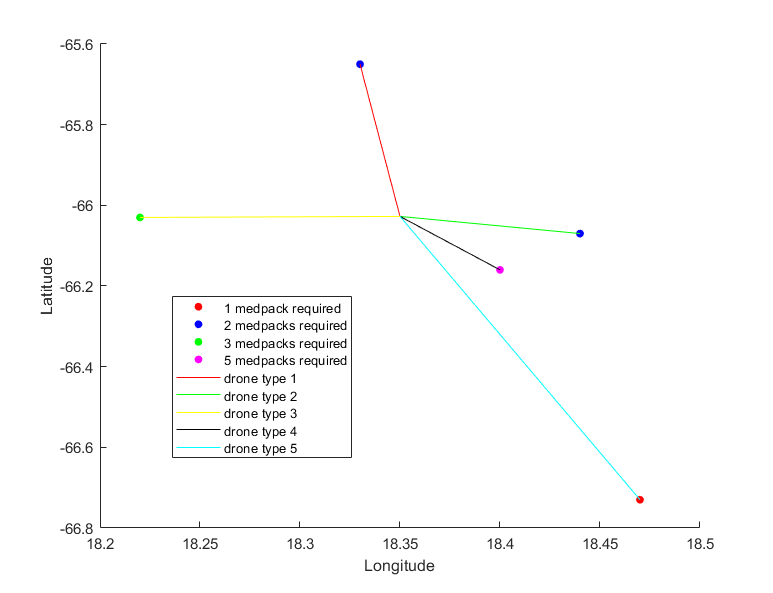
\includegraphics[width=0.7\linewidth]{../example_flight_plan}
	\caption[Fig 1.]{Example optimized flight plan, ran with drone fleet size of 5, starting location 1, 5 allowed movements, and $\gamma$ = 2}
	\label{Fig 1.}
\end{figure*}

\subsection{Parameter sensitivity}
The model output, specifically the outputs of the cost function were analyzed after varying different parameters to find reasonable values for further analysis. There values were the different valid storage bin configurations, the number of allowed movements in a flight plan and the number of drones in a fleet.



\end{document}
